%\section{Outline}

\section{Variables}
To be able to simulate the spread of COVID-19, we have to break the things which affect it down into tangible variables. Some of these variables can then later be selected to be used in the simulation. The criteria for the variables are that they have to be realistic for us to simulate and they have to be relevant in terms of the problem statement. These variables that will be covered and described in this section are the virology of SARS-CoV-2, societal factors that enables the spread of the virus, as well as preventative measures that intent to limit the spread of the virus.

%%HUSK - Virology skal komme først (Gilberto 4. møde)

\subsection{Societal factors}
There are lots of different societal factors that can affect the spread of a virus, such as the living conditions of an area. This could be socioeconomic status, the population density, sanitary facilities and so on. Although we recognize the validity of the aforementioned factors, we will primarily focus on the population density as an important factor.\\
Another societal factor to consider is the culture of a designated country or area, since the spread of the virus is highly dependant on how we interact with each other.



\subsubsection{Population Density}
Population density is an important factor to consider when estimating the spread of a virus, such as COVID-19. This is both in terms of the total number of contacts a person has as well as the spread- and decay duration of the disease. \\
The population density has an effect that is proportional to the contact rate \citep{rocklov_high_2020} in terms of the total number of contacts. This means that it would take less time for the disease to spread in a densely populated area. This in turn ties into the population density's effect on the spread and decay duration.
\begin{figure}[H]
    \centering
    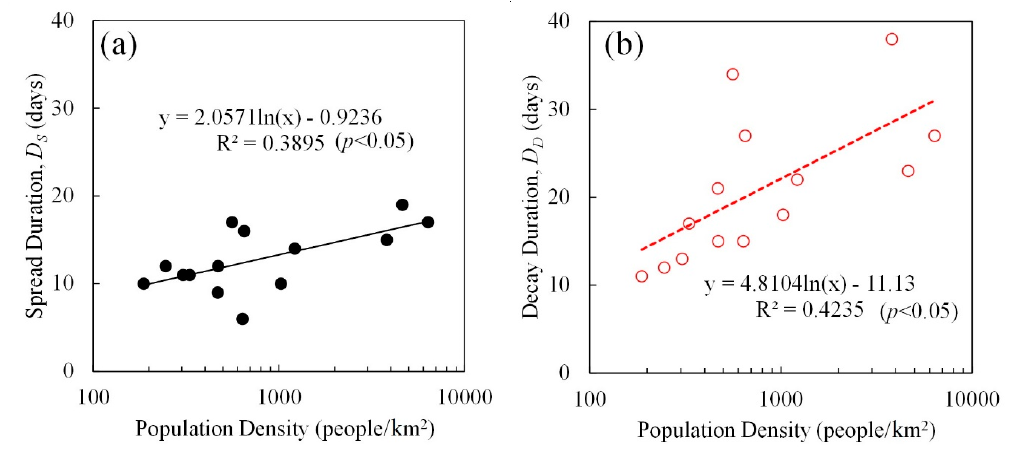
\includegraphics[width=0.8\textwidth]{0_billeder/Spread-Decay.png}
    \caption{``Relationship of the (\textbf{a}) spread and (\textbf{b}) decay durations ($D_S$ and $D_D$) with population density.'' \citep{rashed_influence_2020}}
    \label{fig:Spread-Decay}
\end{figure}
In this study, different districts in Japan with different population densities were chosen and studied, in figure \ref{fig:Spread-Decay}. The data from these districts have been plotted. There is an observable trend in this figure, which shows that population density also has a considerable effect on the spread and decay duration of COVID-19 outbreaks. 



\subsubsection{Culture}
Since it has now been established that one of the main dangers of COVID-19 is how many people are gathered in a given location, cultural differences between peoples must be considered a parametre that - if nothing else - needs mentioning.

In this report, we will use the term "culture" as an umbrella term that encompasses both special occasions (Chinese New Year, American Thanksgiving and the like) and the more general way that people intermingle in their society. It should here be mentioned that scholars like Yoosefi Lebni et al. have pointed out that the cultural aspect also includes the willful endangerment of others by some people to ensure their own survival \citep{yoosefi_lebni_how_2020}. In the context of COVID-19, this cultural aspect relates specifically to hoarding and looting to ensure food and water for oneself and one's family.

Bruns et al. have pointed out that COVID-19 has also greatly influenced different aspects of culture, such as greetings, major holidays and events, and interactions between family members and friendship groups \citep{bruns_covid-19_2020}. Because culture is such a vague entity, it is hard to quantify within the context of a simulation.



\subsection{Virology of SARS-CoV-2}

The virology of SARS-CoV-2 is not a field, where any conclusions can be seen as being final, as it continuously gets updated when new discoveries are made, and thereby having the chance of making past conclusions invalid.

The incubation period (the time from exposure to symptom onset) is set to be about 10 - 14 days, though the more standardized incubation period is set to be 14 days. From the onset of symptoms, and 10 - 14 days forward (20 days for immunocompromised, or in severe cases of COVID-19), the person infected would be contagious. How contagious a person is vary from the level of the symptoms the infected has. \citep{ries_how_2020}

So far there hasn't really been any studies on why, if or how the following variables affects the spreading of SARS-CoV-2:
\begin{itemize}
  \item Age
  \item Gender
  \item immunocompromisation
  \item Pregnancy
\end{itemize}

Though, some of the variables can be used to determine how bad an individual will be affected by COVID-19. As there is loads of studies on how the different variables determine if you will have a severe case of COVID-19.

Age (age groups) and immunocompromisation can be used as a factor for determining if the individuals will have a severe case of COVID-19, and if it will be leading to death. Genderwise, the number of men who dies from COVID-19 is 2.4 times that of women,independent of age \citep{jin_gender_2020}. With pregnancy, the studies that has already been done, haven't lead to any evidence on COVID-19 having any effect on the pregnancy, neither on the fetus during pregnancy or post-birth.


\subsection{Preventive measures}
It is impossible to debate the spread of COVID-19 without including the numerous and different preventive measures that have been implemented both within countries and states as well as across borders. As COVID-19 can be a potentially catastrophic, global event if no preventive or mitigative measures are implemented, it is also relevant to outline several types of preventive measures. Preventive measures can be implemented by the individual, a group of individuals or a governing authority.

We aim to use our model to compare and contrast different preventive and mitigative measures to simulate COVID-19. Therefore, a comprehensive outline of the many preventive measures that have been implemented within Denmark is needed. In this section, we will outline many different factors that aid prevention of COVID-19 with the goal of implementing variables into the simulation that are relevant and plausible. While all the mentioned preventive measures might not be used for the final simulation, this will make it possible for us to argue why we might leave some out.


\subsubsection{The insecurity of social responsibility}

At the core of any preventive measure that spans an entire society, whether local, regional or even global, is of course individual, social responsibility. In short, it is always up to the individual to adhere to the rules put in place by the relevant authorities. A comprehensive overview of mitigative measures that can be implemented by the individual is found in \textit{COVID-19 (SARS-CoV-2) pandemic: fears, facts and preventive measures} \citep{ayenigbara_covid-19_2020}, who have also created figure \ref{fig:Mitigative-Measures}. These mitigative measures all start with the individual’s own will to comply with them. Therefore, many of the preventive and mitigative measures mentioned in this report will be based - at least in part - on this figure.

\begin{figure}[H]
    \centering
    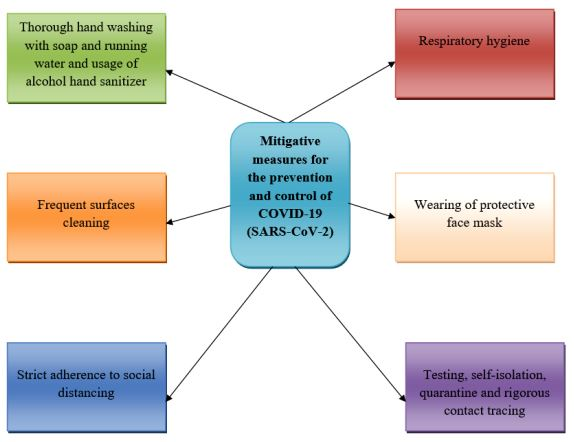
\includegraphics[width=0.75\textwidth]{0_billeder/mitigation of COVID-19.JPG}
    \caption{Mitigative measures that should be implemented across a society to combat COVID-19 \citep{ayenigbara_covid-19_2020}}
    \label{fig:Mitigative-Measures}
\end{figure}

Here, a note of definitions must be made. The word "mitigative" is of course not the same as the word "preventive". Mitigative actions are not, per se, actions that can completely prevent the transmission of COVID-19, but rather minimize the risk of rampant spread. When discussing an illness like COVID-19, a realistic view is important, and unfortunately, it is more realistic to focus on mitigative.

\textit{and} preventive measures than purely on preventive measures.

As social responsibility relies heavily on every single individual in a given, geographical location, this parametre must be considered relatively insecure in nature. Therefore, social responsibility as a factor has been parted into the following multiple parametres to ensure minimal insecurity for each.



\subsubsection{Hygiene}

As shown in figure \ref{fig:Mitigative-Measures}, hygienic prevention is key for the individual to prevent spread of COVID-19 and ensure the safety of both themselves and others. Four of the six mentioned mitigative measures relate to personal hygiene or cleanliness of environment (hand-washing, respiratory hygiene, mask-wearing, and surface-cleaning). For this report, we will consider respiratory hygiene measures as an umbrella term underneath which mask-wearing is the main component, as humans tend to breathe more often than they cough or sneeze.



\subsubsection{Mask-wearing}

A popular means of prevention against COVID-19 amongst civilians and medical personnel alike has been the usage of face masks and shields. Ayenigbara et al. define a protective face mask as a mask made of ``protective materials used to cover the nose and mouth in order to prevent the spread of highly infectious respiratory deseases like influenza, MERS and COVID-19.''\citep{ayenigbara_covid-19_2020}. Wearing protective face masks are particularly helpful in minimizing risk of transmission via droplets, one of two main methods by which the virus spreads.

Wearing masks is particularly useful in minimizing the spread from persons who have tested positive to other persons \citep{ayenigbara_covid-19_2020}. It should be noted that wearing the mask whilst uninfected will also reduce risk of transmission. In short, wearing a mask both mitigates the general spread and the individual's risk of infection.



\textbf{Other respiratory hygiene measures}

Other than mask-wearing, other respiratory hygiene measures can also mitigate spread of COVID-19. One such example of respiratory hygiene is sneezing and coughing into something that can preferably be immediately disposed of, such as tissue paper. Generally, minimizing the transmission of droplets via sneezing and coughing helps mitigate spread of COVID-19, as the virus is considered airborne via droplets \citep{zhang_identifying_2020}. The virus' status as purely airborne is questioned by some scholars, such as Ayenigbara \citep{ayenigbara_covid-19_2020}, so this report will consider COVID-19 only airborne via droplets.




\subsubsection{Hand sanitizer and other hygienic measures}
While COVID-19 is airborne, it can also be transmitted via physical touching of surfaces or substances (and persons) that have been exposed to COVID-19. The risk of infection is highest if the eyes, nose and/or mouth is touched by a surface, substance or person that is in contact or has been in contact with the virulent pathogen known as Sars-Cov-2 \citep{ayenigbara_covid-19_2020}. As explained previously [SOMEONE EXPLAIN THIS PREVIOUSLY], Sars-Cov-2 is the pathogen that leads to the illness known as COVID-19 or, in layman's terms, coronavirus.

Since Sars-Cov-2 is a highly contagious pathogen, it is important to maintain a high level of personal hygiene as well as hygiene in one's surroundings to minimize the risk of transmitting COVID-19. One obvious instance is through the rigorous usage of hand sanitizer and frequent hand-washing. To be at all effective, a hand sanitizer must be alcohol-based and properly and safely stored \citep{gharpure_knowledge_2020}.

While washing hands is a more thorough (if done correctly) way of preventing transmission of COVID-19, it can also be quite harsh on the skin to frequently use soap and similar cleaners - not to mention improbable in larger, semi-public areas such as supermarkets, schools and corporate workspaces according to \cite{cavanagh_rational_2020}. Therefore, hand sanitizer is the default "on-the-go" method for cleaning hands and thereby minimizing transmission through touching of surfaces. Lastly, each person should aim to touch their face as little as possible throughout their day. This measure will also aid in minimizing risk of infection via one's own mask.




\subsubsection{Social distancing and quarantine}
A parametre that is almost completely up to each individual is social distancing. Social distancing is very simply the act of keeping a physical distance to other persons whilst in public and semi-public scenarios \citep{ayenigbara_covid-19_2020}. Social distancing can be differentiated from quarantine and lockdown with the very simple difference being that social distance is preventive on a smaller scale; each person must make an effort to distance themselves from each other. In comparison, quarantine is the act of self-isolating either individually or as a household.

Measures can be taken to ensure minimal distance between two persons who, for instance, need to be closer than 2 metres to interact in relation to exchange of goods and services. The usage of see-through plastic shields between cashiers and customers in shops is one such example. However, for most instances, social distance should be considered the primary, preventive measure.




\textbf{Quarantine or self-isolation}

Quarantine is not a preventive measure if we assume what is to be prevented is illness. However, when it comes to a pandemic, society at large must aim to prevent further spread of the illness in question. Quarantine is a state of living that a person enters once they have been infected with this illness - in this case COVID-19. Quarantine can hereby become a preventive measure on a larger scale; when sectioning off persons infected with COVID-19, you prevent further transmission to others. During the international COVID-19 crisis, the word "self-isolation" has also been used to explain this state of living. In this report and context, the two terms are considered synonymous, regardless of etymological differences and historical applications.

As opposed to social distance, once a person has entered quarantine, they are not to interact with anyone – including within their own household. If the layout of the home permits it, they should stay completely separate from the rest of the persons living with them, and cleaning should be a focus to ensure minimal risk of spreading via surfaces (furniture and the like) \citep{ayenigbara_covid-19_2020}. If an entire household self-isolates together, these measures can of course be done away with entirely. Regardless of whether a person is self-isolating by themselves or their family, the point is to do away with contact with others to the best of the person's (or persons') ability.




\subsubsection{Assembly ban and lockdown}

Although both assembly ban and lockdown can be considered part of social distance, there are some defining, differing factors. Firstly, an assembly ban is simply the governmentally implemented ban on assemblies (meaning social groups) that exceed a certain number. For instance, in March 2020, assemblies exceeding 100 people were banned by the government in Denmark \citep{ronnstad_tidslinje_2020}. 




\textbf{Assembly ban}

Banning larger gatherings and social assemblies does not target specific social groups, religious groups or political groups when it is done as a preventive measure against pandemics. As such, while assembly bans can normally be quite polarising and controversial, they have been largely accepted by general publics across the world \citep{gostin_governmental_2020}. 

Assembly bans can, as mentioned, be given a quantifier in the form of an upper limit of individuals in a given group. This quantifier is chosen by the relevant authorities, which are Statens Serum Institut in Denmark's case. 

In March 2020, an assembly ban was introduced to Denmark. In the following five months, the assembly ban fluctuated between a maximum of 1,000 people to a maximum of just 10 people. As of the 23rd of October 2020, following a second wave of COVID-19 infections in the country, Denmark has a temporary assembly ban of 10 people or more \citep{ronnstad_tidslinje_2020}.




\textbf{Nationwide lockdown}

Several nations have found it necessary to implement nationwide lockdowns to combat the spread of COVID-19. China, Italy and the state of New York in the United States of America have all used some kind of lockdown to mitigate the virus spreading. The effects of these lockdowns can be seen in figure \ref{fig:Confirmed-infections-international} of confirmed infections \citep{zhang_identifying_2020}.

\begin{figure}[H]
    \centering
    \includegraphics[width=0.75\textwidth]{0_billeder/Confirmed infections international.JPG}
    \caption{Comparison of infection trends between Wuhan province, New York State and Italy including when lockdown and similar preventive measures were implemented.
    \citep{zhang_identifying_2020}}
    \label{fig:Confirmed-infections-international}
\end{figure}

As shown in figure \ref{fig:Confirmed-infections-international}, the steady increase in confirmed infections was curbed after implementing either a temporary lockdown, stay-at-home orders or social distancing. Lockdowns can be considered the most serious implementation of what is, at its core, a form of social distancing. 

When a lockdown is implemented, schools and non-essential businesses are typically closed and assembly bans are implemented. Depending on severity of the infection rate, stay-at-home orders and curfews can also be implemented. Lastly, quarantines for inbound travelers or actual bans on inbound travelling can also be implemented as part of nationwide lockdown \citep{gostin_governmental_2020}.




\subsubsection{Information and misinformation}

General information given to both the general public and lesser authorities within a society regarding COVID-19 is one of the most effective ways to minimize further spread of the illness. Although misinformation is of course not a preventive measure, it is a large enough factor within prevention of COVID-19 to warrant a few words on the topic. In the modern day, a lot of information can be given to the general public digitally, such as through apps and websites. This will be further outlined in subchapter \ref{Contact Tracing}.

Bierwiaczonek, Kunst and Pich have already concluded that conspiracy theories surrounding COVID-19 reduces social distancing \citep{bierwiaczonek_belief_nodate}, and Tasnim et.al have similarly concluded that the general spread of misinformation hinder the mitigation of COVID-19 on both a local and global scale \citep{tasnim_impact_2020}. Lastly, Pennycook et.al. have paid special attention to how this misinformation especially spreads on social media (Facebook, Reddit, YouTube and the like) \citep{pennycook_fighting_2020}. It can therefore confidently be stated that misinformation can be detrimental to the general prevention of COVID-19 and similar, respiratory infections.




\textbf{Trust in authority}

A major authority of COVID-19 and similar health topics that span the globe is the World Health Organization \citep{who_home_nodate}. WHO collects data about transmission, recovery rates, morbidity, and the like. They also inform the general, international public about precautionary measures each individual can make use of to minimize risk of infection for both themselves and their family. 
For Denmark specifically, Statens Serum Institut (SSI) is another authority. SSI is an institute that operates under the Danish Ministry of Health. SSI is one of the main sources this paper have used to collect raw data of transmission and day-by-day development of the virus’ spread within the country \citep{ssi_statens_nodate}.




\subsubsection{Contact Tracing} \label{Contact Tracing}
With COVID-19 being easily spread from one person to another, it is important to identify, who a person (who have tested positive) have been in contact with, within the time period that they could have spread the virus to other people. These people are called contacts, and will be observed for two weeks, to see if they develop any symptoms, and if so, if they have contracted the virus. The goal of course is to minimize the spread of COVID-19 pandemic.\citep{who_hq_coronavirus_2020}
The World Health Organization have written about the several steps of contact tracing.\newline
First of all, contacts needs too be defined, who is considered a contact? In the case of COVID-19 the definition of a contact is: "a contact is a person who has been exposed to someone else infected with the virus that causes COVID-19, from 2 days before to 14 days after the person started to show symptoms."\citep{who_headquarters_coronavirus_2020}\newline
Secondly the defined contacts needs to be identified. Here the infected person will be interviewed, to fin out who they have had contact with.\newline
Thirdly the identified contacts should be contacted to inform them, to let them know that they have been contact traced and what the purpose of contact tracing is, and how their personal data is used.


There are different methods of... smitte|stop

\section{Scope}

When discussing simulations and COVID-19 disease in general, there are several options regarding the scope of the project, including the simulation and data collection needed to determine different tasks. The scope of the project is a major part of the planning process, which determines key aspects such as the size of the problem, documenting variables and specific goals necessary to keep deadlines.
The scope of the project can generally be seen as a mixture of gathering information and process planning, where the members "scope out", i.e. plans ahead of the operation in a broader sense, and trying to identify the workflow as much as possible. \newline
Large project scopes tend to have more naturally occurring changes due to the natural progression of the project, but if the scoping from the beginning has been effective, it will also be easier for the members to adapt to these changes. An initial scoping of the project is necessary to continue on with a problem analysis and determine the key areas. In other words, there must be some form of general scope of the project before an initial problem analysis can be done.  

When looking at the project of simulating COVID-19, there are also different scopes to describe the size of the simulation. The scopes described here are used as form of indication of how big the simulation will be, and how representative it could be in the real world. 
The four main scopes to look at when discussing a pandemic is the following: 

\begin{itemize}
\item International
\item National
\item Regional
\item Local
\end{itemize}

In this specific project of simulating COVID-19 and the technology contract tracing, the main focus will be on the local and regional scope. Due to the natural limitation of the project hence inexperienced members, lack of time, minimal funding etc., the decision has been made to focus mainly on the local and regional scope. Included in this decision were key factors such as the observation of daily foot traffic at specific times, how preventative measures affects human behaviour and how the technology \textbf{contact tracing} works in reality. For the group to make a reasonable product of a simulation with these natural limitations, it came clear early in the process that the scope of the project should be no bigger than regional, if the group were to give a satisfying result. 

For the initial rounds of brainstorming, our focus was therefore very heavily on prevention and mitigation, as we considered contact tracing to be a mitigating factor at the very least. We also had personal interest in areas in our immediate vicinity with high foot traffic. As we live in Aalborg, we knew we wanted to focus on Aalborg, but we were not yet certain whether to focus on just Aalborg as a whole or a specific area of Aalborg. There was particular interest in simulating Jomfru Ane Gade, a walking street that is famous for being made up completely of bars, discos and similar establishments.

Our initial interest in this area was focused on the pure chaos associated with the location. The inebriation that surrounds the area made it interesting to try to simulate, but it also posed many different challenges. Instead, we decided to focus our simulation on just Aalborg, as there are clearer data to build a model on.


